\item Un fabricante de cartuchos para equipos estereofónicos diseñó una aguja con una sección transversal parabólica, como se ilustra en la figura. La ecuación de la parábola es $y = 16x^2$, en donde $x$ y $y$ se miden en milímetros. Si la aguja se posa en un zurco de disco cuyos lados forman un ángulo $\theta$ con la dirección horizontal, en donde $\tan \theta = 1.75$, encuentre los puntos de contacto $P$ y $Q$ de la aguja con el surco.
    
    \begin{center}
    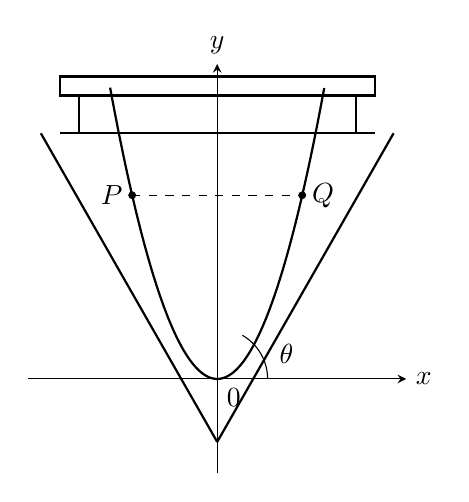
\begin{tikzpicture}[scale=0.8]
        \draw[-stealth] (-3,0) -- (3,0) node[right] {$x$};
        \draw[-stealth] (0,-1.5) -- (0,5) node[above] {$y$};
        \draw[thick, domain=-1.7:1.7, samples=100] plot (\x, {1.6*\x*\x});
        \draw[thick] (0,-1) -- (2.8, 3.9);
        \draw[thick] (0,-1) -- (-2.8, 3.9);
        \filldraw[fill=black] (1.35, 2.916) circle (1.5pt) node[right] {$Q$};
        \filldraw[fill=black] (-1.35, 2.916) circle (1.5pt) node[left] {$P$};
        \node[below right] at (0,0) {$0$};
        
        \draw[thick] (-2.5, 4.5) rectangle (2.5, 4.8);
        \draw[thick] (-2.2, 3.9) -- (-2.2, 4.5);
        \draw[thick] (2.2, 3.9) -- (2.2, 4.5);
        \draw[thick] (-2.5, 3.9) -- (2.5, 3.9);
        
        \draw[dashed] (-1.35, 2.916) -- (1.35, 2.916);
        \draw[dashed] (0,-1) -- (0,0);
        \draw (0.8,0) arc (0:60:0.8);
        \node at (1.1,0.4) {$\theta$};
    \end{tikzpicture}
    \end{center}
